\chapter{Case study}\label{chap:case}
Dynamic languages with a garbage collector have the advantage of letting the programmer use the exploratory style of programming, where he doesn't have to worry about memory management or other low level considerations. [][] Doesn't have to design a complex type hierarchy or any similar scaffolding. He can just jump in and start implementing an idea. This is excellent for prototyping.

But when it comes to performance and robustness this approach shows its downsides very quickly. The safety of static types combined with a good development environment catches a lot of bugs and inconsistencies before runtime. Garbage collector mechanisms vary in implementation, each showing a different performance characteristic. In this chapter I will describe the implementation of a clone of Pac-Man in Dual and performance issues that I've encountered. These are very much related to the JavaScript environment, notably the event loop and the garbage collector, which has different implementations across browsers. The latter did shows a significant difference when comparing different web browsers.

Implementation of a non-trivial application allows to test the language design and quickly establish which features are the most useful in practice.
I found that I could do away with a lot of the more complex ones %% performance gain, net win

\section{The game}
It is actually a port of my earlier clone of the game, which was written in Links\footnote{\url{http://groups.inf.ed.ac.uk/links/}}, a functional language.

\begin{figure}[h!]
\centering
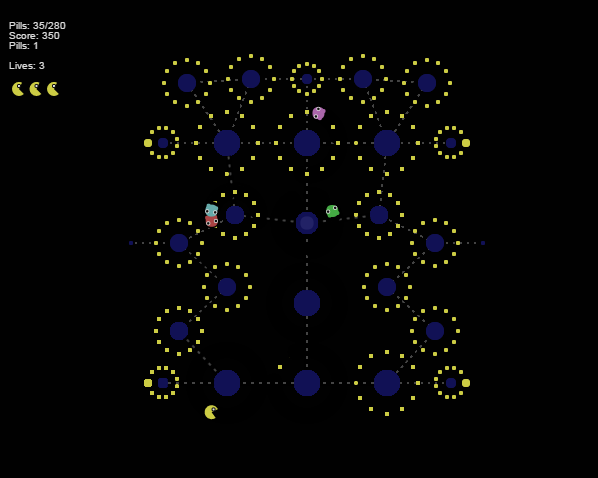
\includegraphics[width=0.9\textwidth]{pacman}
\caption{A screenshot from the game}
\label{fig:pacman}
\end{figure}

\subsection{Main loop}
A typical game loop in a modern JavaScript game\footnote{\url{https://developer.mozilla.org/en-US/docs/Games/Anatomy}} relies on the \texttt{requestAnimationFrame} method\footnote{\url{https://developer.mozilla.org/en-US/docs/Web/API/Window/requestAnimationFrame}}. This method takes a single argument, which is a function callback. This function is invoked by the browser before it repaints the contents of the window. Thus, it allows the game rendering to be synchronized with the browser.

The callback invoked by \texttt{requestAnimationFrame} receives a timestamp, specifying the time of the repaint event. Ideally and under the most common circumstances this happens 60 times a second.

I implemented the game loop in Dual as follows:
\begin{lstlisting}
-- [1] the amount of milliseconds between
--        game state updates:
bind [tick-length 50]

-- the main loop function:
bind [main-loop
-- arguments:
--    game-state -- current game state
--    last-tick -- time of the last
--        game state update
--    fps-info -- an object used for debugging,
--        which contains information about
--         the frame rate
--     current-time -- the time of  the current
--        invocation of the loop
of [game-state last-tick fps-info current-time do [
    -- [2] schedule the next iteration of the loop
    --        using requestAnimationFrame:
    async [
        .[window requestAnimationFrame]
        of [next-time
            main-loop[
                game-state
                last-tick
                fps-info
                next-time
            ]
        ]
    ]
    
    -- the timestamp of the tick after the last tick
    bind [next-tick +[last-tick tick-length]]
    
    -- counts how many state updates should be
    --        performed in this iteration:
    bind [tick-count 0]
    
    -- if the current time is past the timestamp of
    --        the next tick, the above counter
    --        should be incremented;
    -- possibly more than by one, if the difference
    --        is a multiply of tick-length
    if [>[current-time next-tick] do [
        bind [time-since-tick
              -[current-time last-tick]]
        mutate [
            tick-count
            .[math floor][
                /[time-since-tick tick-length]
            ]
        ]
    ] false]
    
    -- perform the calculated amount of
    --        game state updates:
    bind [i 0]
    while [<[i tick-count] do [
        -- keep track of the time of the last tick:
        mutate [last-tick +[last-tick tick-length]]
        
        -- invoke the function that updates
        --        the game-state:
        mutate [
            game-state
            main-game-logic[game-state input-queue]
        ]
        mutate [i +[i 1]]
    ]]

    -- if there were game state updates,
    --        redraw game screen; else do nothing:
    if [>[tick-count 0]
        mutate [fps-info draw[
            game-state
            current-time
            .[window performance now]!
            fps-info
        ]]
        _
    ]
]]]
\end{lstlisting}


\section{Performance}
Disparity between Firefox and Chrome, reflecting differences in garbage collector implementations.

Issue: interpreter is blocking the event loop.
There's a lot of intermediate objects created that have to be garbage collected.

\begin{figure}[h!]
	\centering
	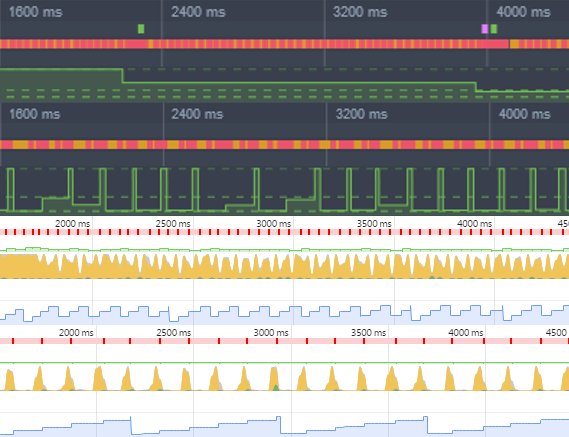
\includegraphics[width=0.9\textwidth]{profiling}
	\caption{Comparison of Firefox' and Chrome's profiler outputs}
	\label{fig:profiling}
\end{figure}

General pattern:
Chrome more frequent garbage collections
more regular
more predictable

Details are a topic for another thesis

\section{Possible improvements}
Interruptable eval

Continuation-passing style
State machine
Anyway, explicit stack

Additional benefits:
	can pause and debug the application, step through
	can record the state and rewind